\documentclass[./main.tex]{subfiles}

\begin{document}
\newpage
\chapter*{Appendix}
\addtocontents{lof}{\protect\addvspace{-10pt}}
\section*{Data Scraping Code }
\begin{lstlisting}[frame=single, language=python,basicstyle=\small\ttfamily,breaklines=true,showspaces=false,columns=fullflexible, literate={\ }{{\ }}1]
from bs4 import BeautifulSoup
import requests
import csv
# Site Url
URL = "https://merolagani.com/LatestMarket.aspx"
# make get request to fetch the raw html content
conn = requests.get(URL)
soup = BeautifulSoup(conn.text, 'lxml')
table = soup.find('table', class_='table table-hover live-trading sortable')
headers = [i.text for i in table.find_all('th')]
print(headers)
data = [j for j in table.find_all(
    'tr', {"class": ["decrease-row", "increase-row", "nochange-row"]})]
result = [{headers[index]: cell.text for index,
           cell in enumerate(row.find_all('td'))} for row in data]
# writing the data in CSV file with headers and their respective values
with open('nepse.csv', 'w') as f:
    try:
        writer = csv.DictWriter(f, fieldnames=headers)
        writer.writeheader()
        writer.writerows(result)
        print("CSV file created successfully and data written successfully")
    except Exception as e:
        print(e)
f.close()
\end{lstlisting}
\newpage
\section*{Symbol Data Scraping Code }
\begin{lstlisting}[frame=single, language=python,basicstyle=\small\ttfamily,breaklines=true,showspaces=false,columns=fullflexible, literate={\ }{{\ }}1]
from selenium import webdriver
from selenium.webdriver.chrome.options import Options
from bs4 import BeautifulSoup
from selenium.webdriver.common.by import By
import time
import csv
StockSymbol = input("Enter the stock symbol: ")
time.sleep(2)
driver = webdriver.Chrome()
url = f"https://merolagani.com/CompanyDetail.aspx?symbol={StockSymbol}#0"
driver.get(url)
print (" ......... Fetching Data From Merolagani ............ ")\
button = driver.find_element(By.XPATH,
    '//*[@id="ctl00_ContentPlaceHolder1_CompanyDetail1_lnkHistoryTab"]'
)
button.click()
time.sleep(2)
page_source = driver.page_source
soup = BeautifulSoup(page_source, 'html.parser')
table = soup.find_all('table', class_='table table-bordered table-striped table-hover')
headers = [i.text.replace('\n', '') for i in table[0].find_all('th')]
print(headers)
data = [[i.text for i in row.find_all('td')] for row in table[0].find_all('tr')]
driver.quit()
print(" ......... Generating CSV File OF Company Data ............ ")
time.sleep(2)
try:
    with open(f'{StockSymbol}.csv', 'w', newline='') as file:
        writer = csv.writer(file)
        writer.writerow(headers)
        writer.writerows(data)
        print("Done")
except Exception as e:
    print(e)
    print("Error in generating CSV file")

\end{lstlisting}
\newpage
\section*{Stock Price Prediction Code}
\begin{lstlisting}[frame=single, language=python,basicstyle=\small\ttfamily,breaklines=true,showspaces=false,columns=fullflexible, literate={\ }{{\ }}1]
"""
Importing Libraries
"""
import pandas as pd
import numpy as np
from sklearn.preprocessing import MinMaxScaler
from tensorflow.keras.models import Sequential
from tensorflow.keras.layers import LSTM, Dense
import matplotlib.pyplot as plt
""" 
Loading CSV Data File 
"""
file_path = 'NABIL.csv'
df = pd.read_csv(file_path)
#remove missing valuse 
df = df.dropna()
#scaling data using min-max scaler
scaler = MinMaxScaler()
df_scaled = scaler.fit_transform(df[['Open']])
#Create Dataset
def create_dataset(df_scaled, look_back=1):
  x_train = []
  y_train = []
  for i in range(len(df_scaled) - look_back):
    x_train.append(df_scaled[i:i + look_back])
    y_train.append(df_scaled[i + look_back])
  return x_train, y_train
#
sequence_length = 10
X, y = create_dataset(df_scaled, sequence_length)
train_size = int(len(X) * 0.8)
X_train, X_test = X[:train_size], X[train_size:]
y_train, y_test = y[:train_size], y[train_size:]
model = Sequential()
model.add(LSTM(50, activation='relu', return_sequences=True, input_shape=(sequence_length, 1)))
model.add(LSTM(50, activation='relu'))
model.add(Dense(1))
model.compile(optimizer='adam', loss='mse')
# Convert lists to arrays and reshape for LSTM input
X_train = np.array(X_train).reshape((len(X_train), sequence_length, 1))
X_test = np.array(X_test).reshape((len(X_test), sequence_length, 1))
y_train = np.array(y_train).reshape((len(y_train), 1))
y_test = np.array(y_test).reshape((len(y_test), 1))
model.fit(X_train, y_train, epochs=300, batch_size=32, validation_data=(X_test, y_test), verbose=2)
# Make predictions
train_predictions = model.predict(X_train)
test_predictions = model.predict(X_test)
# Inverse transform the predictions to the original scale
train_predictions = scaler.inverse_transform(train_predictions)
y_train_original = scaler.inverse_transform(y_train.reshape(-1, 1))
test_predictions = scaler.inverse_transform(test_predictions)
y_test_original = scaler.inverse_transform(y_test.reshape(-1, 1))
# Plot the results
plt.figure(figsize=(12, 6))
# Plot training data
plt.plot(df.index[sequence_length:sequence_length+train_size], y_train_original, label='Actual Train Data')
plt.plot(df.index[sequence_length:sequence_length+train_size], train_predictions, label='Train Predictions')
# Plot testing data
test_index = df.index[sequence_length + train_size:sequence_length + train_size + len(test_predictions)]
plt.plot(test_index, y_test_original, label='Actual Test Data')
plt.plot(test_index, test_predictions, label='Test Predictions')
plt.legend()
plt.show()
df = df.sort_index(ascending=False)
# Scale the most recent data
latest_data = df.head(sequence_length)
latest_scaled = scaler.transform(latest_data[['Open']])
# Reshape the scaled data
latest_scaled = np.array(latest_scaled).reshape((1, sequence_length, 1))
# Predict tomorrow's price
tomorrow_prediction = model.predict(latest_scaled)
tomorrow_prediction = scaler.inverse_transform(tomorrow_prediction)
print("Tomorrow's predicted price:", tomorrow_prediction[0, 0])
\end{lstlisting}
\section*{Figures and Graphs}
\begin{figure}[H]
    \centering
    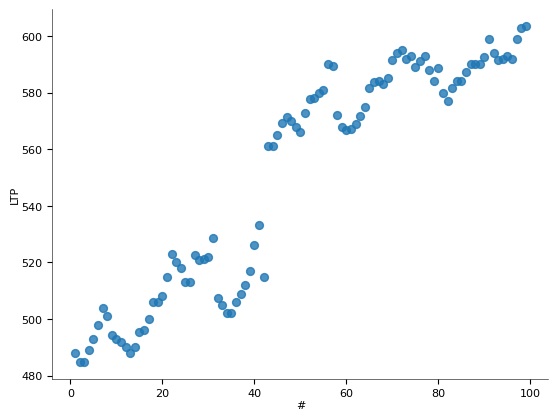
\includegraphics[width=1\linewidth]{images/distribution.png}
    \caption{Data Distribution}
    \label{fig:7.1}
\end{figure}
\newpage
\begin{figure}[H]
    \centering
    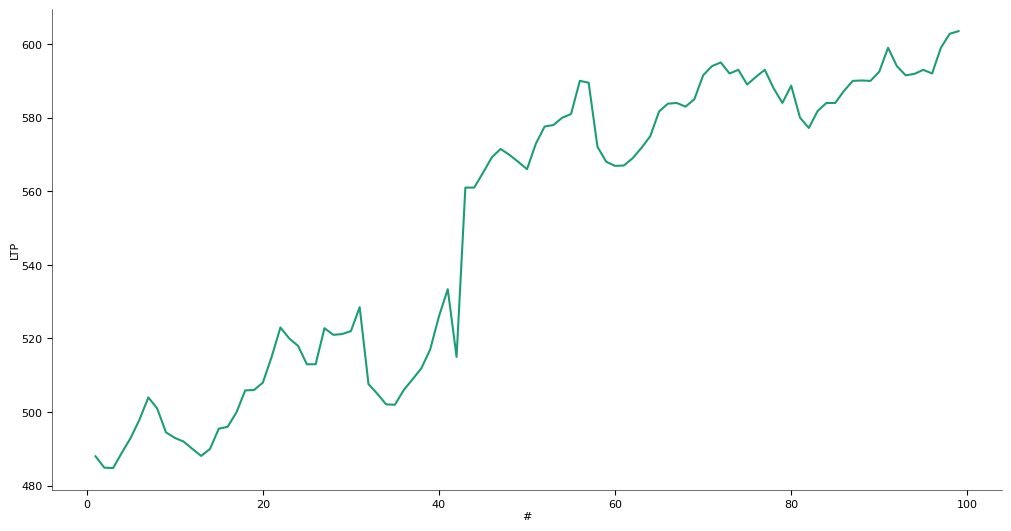
\includegraphics[width=1\linewidth]{images/raw-data-time-series.png}
    \caption{Time series of LTP price}
    \label{fig:7.2}
\end{figure}
\begin{figure}[H]
    \centering
    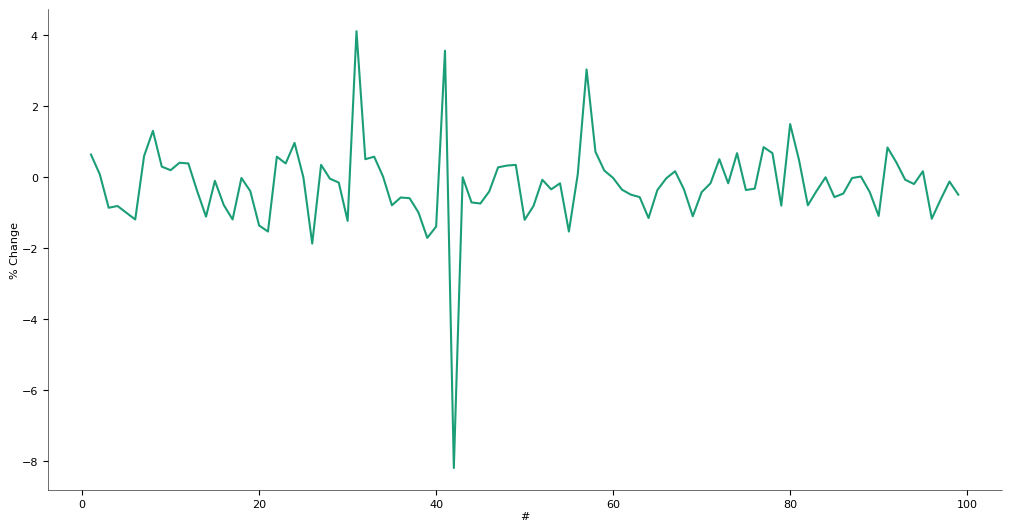
\includegraphics[width=1\linewidth]{images/change-graph.png}
    \caption{Value Change Graph}
    \label{fig:7.3}
\end{figure}
\begin{figure}[H]
    \centering
    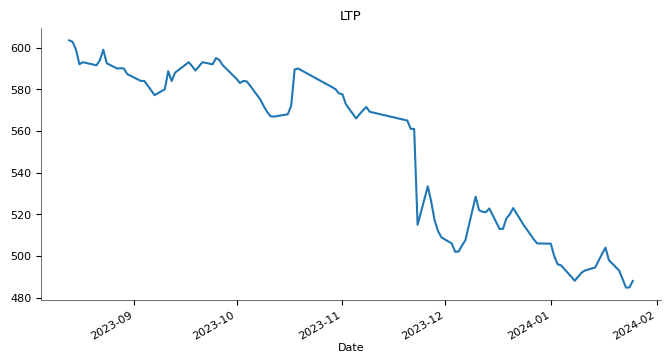
\includegraphics[width=1\linewidth]{images/LTP.png}
    \caption{Time series of LTP}
    \label{fig:7.4}
\end{figure}
\begin{figure}[H]
    \centering
    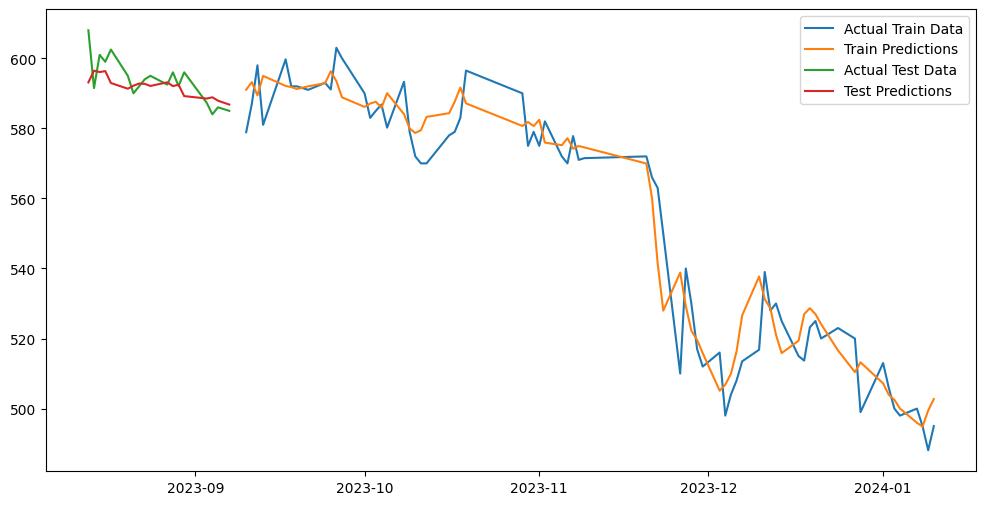
\includegraphics[width=1\linewidth]{images/Trained.png}
    \caption{LSTM prediction}
    \label{fig:7.5}
\end{figure}
\begin{figure}[H]
    \centering
    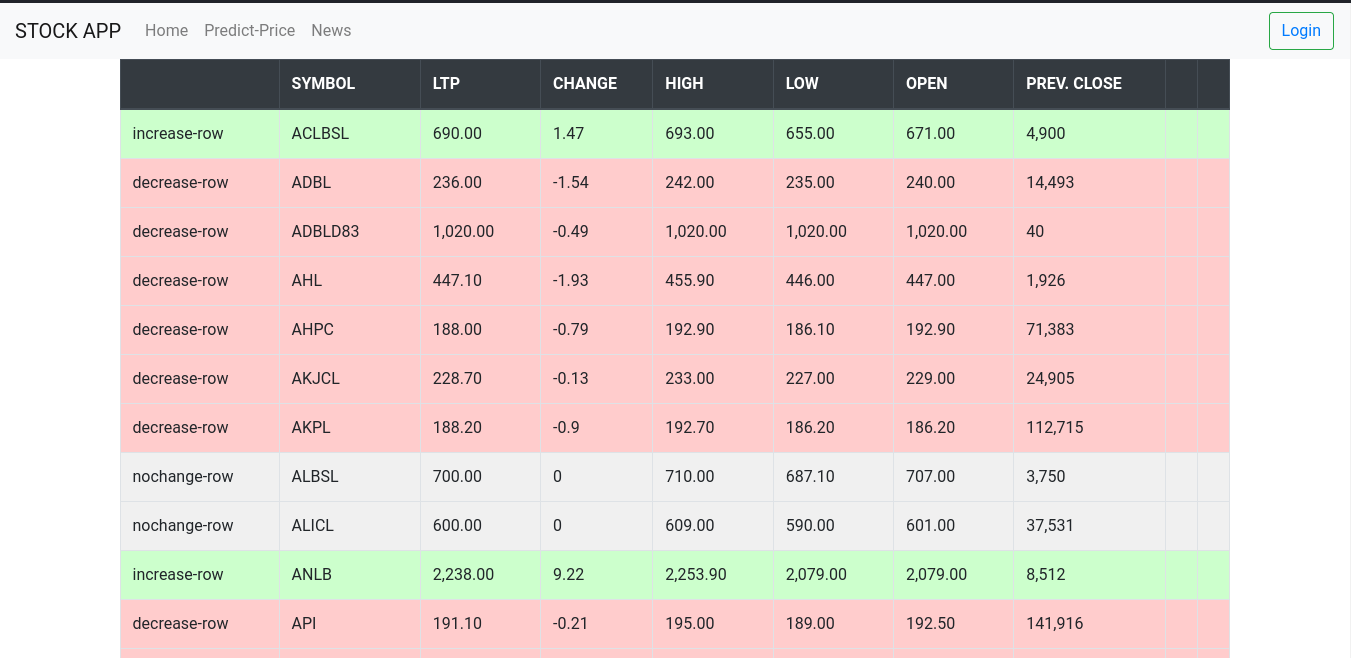
\includegraphics[width=1\linewidth]{images/web1.png}
    \caption{Web Application Home Page}
    \label{fig:7.6}

\end{figure}
\begin{figure}[H]
    \centering
    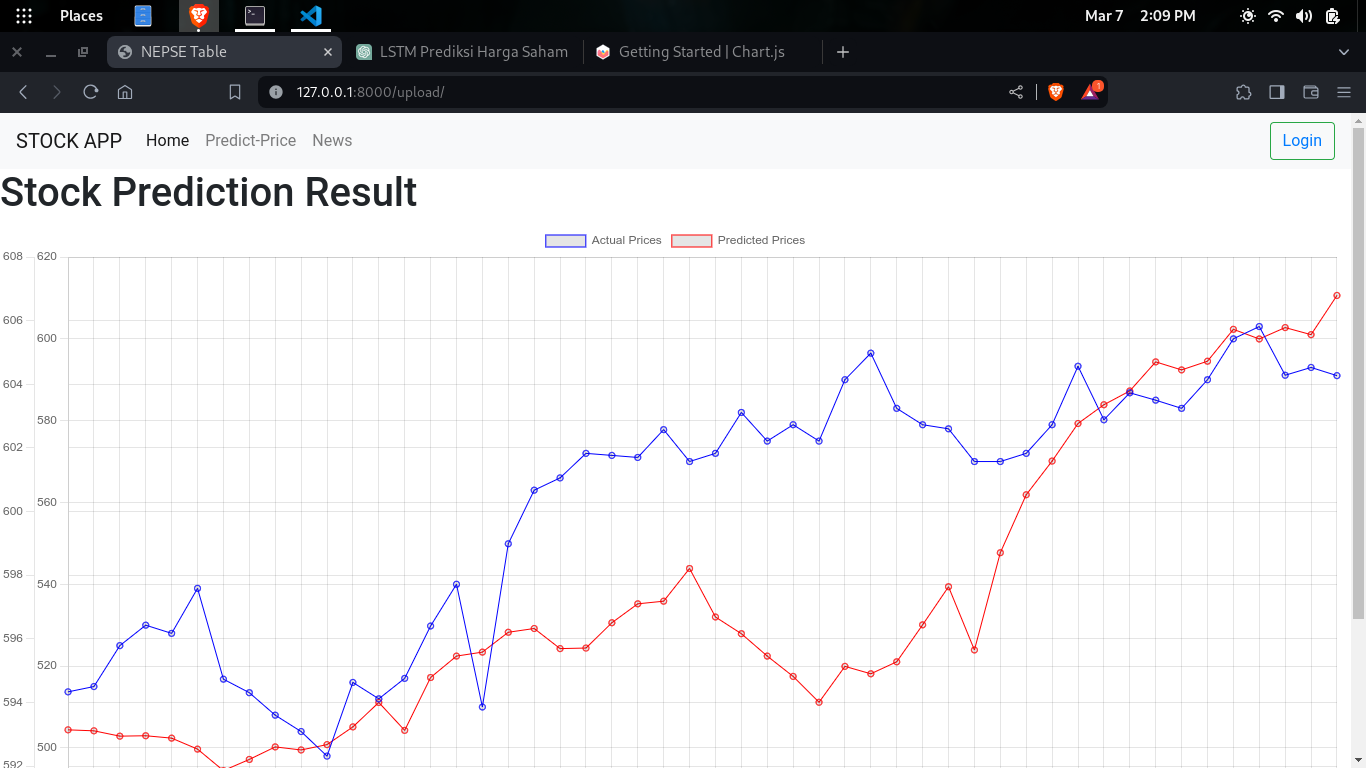
\includegraphics[width=1\linewidth]{images/web2.png}
    \caption{Web Application Data visualization Section}
    \label{fig:7.7}
\end{figure}
\begin{figure}[H]
    \centering
    \includegraphics[width=1\linewidth]{images/web-applicationForm.png}
    \caption{Web Application Form Section}
    \label{fig:7.8}
\end{figure}
\begin{figure}[H]
    \centering
    \includegraphics[width=1\linewidth]{images/web-application-news.png}
    \caption{Web Application News Section}
    \label{fig:7.9}
\end{figure}
\end{document}